\documentclass{article}
\usepackage{tikz}
\usepackage{subcaption}

\begin{document}

\begin{figure}
    \begin{minipage}{0.5\textwidth}
        \centering
        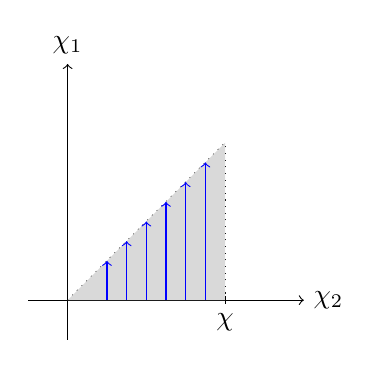
\begin{tikzpicture}[scale=0.5]
            % Draw axes
            \draw[->] (-1,0) -- (6,0) node[right] {$\chi_2$};
            \draw[->] (0,-1) -- (0,6) node[above] {$\chi_1$};
            
             \draw[dotted] (0,0) -- (4,4) node[right]{};
             \draw[dotted] (4,0) -- (4,4) node[right]{};
    
    	      \fill[gray!30] (0,0) -- (4,0) -- (4,4) -- cycle;
	      
              \draw[blue, ->] (1,0) -- (1,1) node[right]{};
              \draw[blue, ->] (1.5,0) -- (1.5,1.5) node[right]{};
	     \draw[blue, ->] (2,0) -- (2,2) node[right]{};
	      \draw[blue, ->] (2.5,0) -- (2.5,2.5) node[right]{};
	      \draw[blue, ->] (3,0) -- (3,3) node[right]{};
	      \draw[blue, ->] (3.5,0) -- (3.5,3.5) node[right]{};

    
            % Draw tick and label for x-coordinate
            \draw (4,0.1) -- (4,-0.1) node[below] {$\chi$};
            
            % Draw frame
        \end{tikzpicture}
        \caption{}
        \label{fig:frame_left}
    \end{minipage}%
    \begin{minipage}{0.5\textwidth}
        \centering
        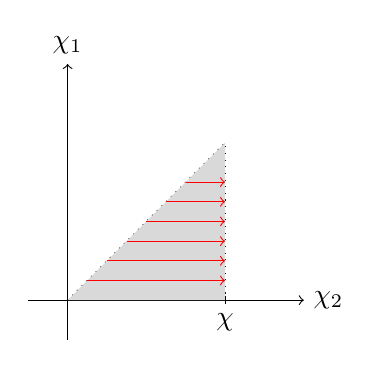
\begin{tikzpicture}[scale=0.5]
            % Draw axes
            \draw[->] (-1,0) -- (6,0) node[right] {$\chi_2$};
            \draw[->] (0,-1) -- (0,6) node[above] {$\chi_1$};
            
             \draw[dotted] (0,0) -- (4,4) node[right]{};
             \draw[dotted] (4,0) -- (4,4) node[right]{};
    
    	      \fill[gray!30] (0,0) -- (4,0) -- (4,4) -- cycle;
	      
	       \draw[red, ->] (0.5,0.5) -- (4,0.5) node[right]{};
              \draw[red, ->] (1,1) -- (4,1) node[right]{};
    	     \draw[red, ->] (1.5,1.5) -- (4,1.5) node[right]{};
              \draw[red, ->] (2,2) -- (4,2) node[right]{};
              \draw[red, ->] (2.5,2.5) -- (4,2.5) node[right]{};
	      \draw[red, ->] (3,3) -- (4,3) node[right]{};

	      
            % Draw tick and label for x-coordinate
            \draw (4,0.1) -- (4,-0.1) node[below] {$\chi$};
            
            % Draw frame
        \end{tikzpicture}
        \caption{}
        \label{fig:frame_right}
    \end{minipage}
    \caption{Two different way of doing the integration of $f(\chi_{1}, \chi_{2})$ over the triangle area, the inner integral is shown in lines. On the left $\int^{\chi}_{0} d\chi_{2} \int^{\chi_{2}}_{0} d\chi_{1}f(\chi_{1}, \chi_{2})$, on the right $\int^{\chi}_{0} d\chi_{1} \int^{\chi}_{\chi_{1}} d\chi_{2}f(\chi_{1}, \chi_{2})$ }  
    \label{fig:frame}
\end{figure}






\end{document}
